\section{Performance Enhancement}



\begin{frame}{A Novel Pre-Processing Method Against Covariate Shift}
    \begin{enumerate}
        \item \textbf{No Prior Shift Knowledge Needed}
        \begin{itemize}
            \item Simplifies implementation by eliminating the need for shift estimation.
            \item Adaptable to various datasets without additional shift information.
        \end{itemize}
        
        \item \textbf{Built-in Regularization}
        \begin{itemize}
            \item Prevents overfitting by introducing controlled noise.
            \item Enhances model generalization on unseen data.
        \end{itemize}
    \end{enumerate}
\end{frame}



\begin{frame}{The R.A.W. Method}
    \begin{columns}[T]

        \begin{column}{0.45\textwidth}
            \vspace{2em} 
                \begin{itemize}\LARGE
                    \item \textbf{R}andom
                    \item \textbf{A}ugmentation
                    \item \textbf{W}alk
                \end{itemize}
   
        \end{column}
        
        \vline\hspace{1em} 
        \begin{column}{0.55\textwidth}
        \begin{figure}
            
            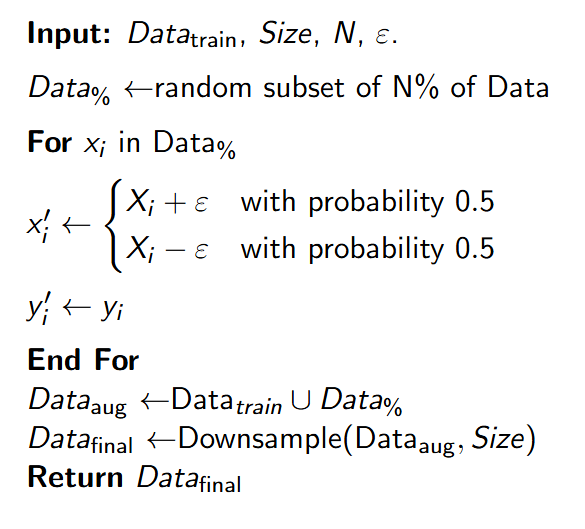
\includegraphics[width=\textwidth]{algo.png}
            
        \end{figure}
        \end{column}
    \end{columns}
\end{frame}


\begin{frame}{Classify With Gradient Boosting Using R.A.W.}
    \begin{enumerate}
        \item  Apply the R.A.W. pre-processing method to the training data to address covariate shift.
        \item  Train a Gradient Boosting Classifier on the augmented dataset.
        \item  Evaluate the model's performance on shifted test sets.
    \end{enumerate}
    
    \vspace{1em}
    \begin{figure}
        \centering
        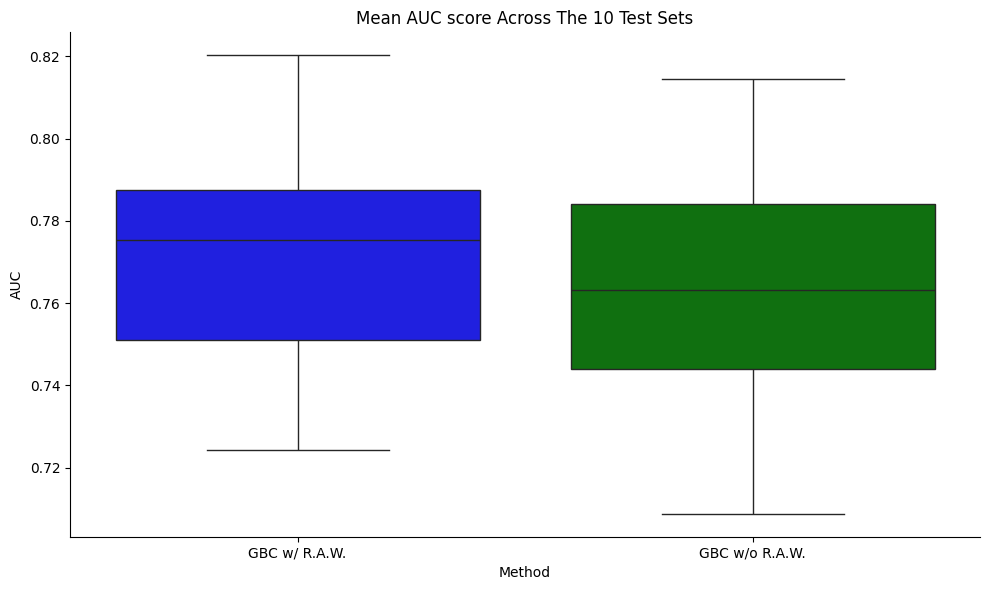
\includegraphics[width=0.49\textwidth]{MeanAUCscoreacross10.png}
        \hfill
        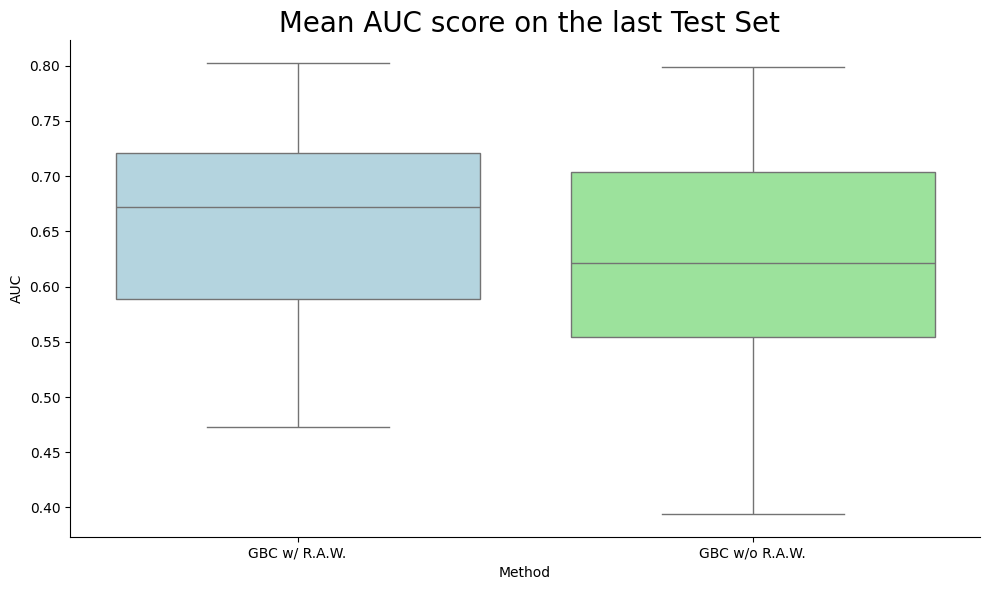
\includegraphics[width=0.49\textwidth]{MeanAUCscoreLAST.png}
    \end{figure}
    
\end{frame}



\begin{frame}{A Statistical Analysis Of The Results}
    \begin{columns}[T]
        \begin{column}{0.59\textwidth}
            \vspace{1em}
            \begin{itemize}
                \item $\boldsymbol{H_0}$: $\Delta\bar{\mu} = \overline{\text{AUC}}_{\text{R.A.W.}} - \overline{\text{AUC}}_{\text{base}} = 0$ \\        
                \item $\boldsymbol{H_1}$: $\Delta\bar{\mu} = \overline{\text{AUC}}_{\text{R.A.W.}} - \overline{\text{AUC}}_{\text{base}} \neq 0$ \\
                \item \textbf{Test:} Paired t-test on 50 independent $\Delta\overline{\text{AUC}}$.
            \end{itemize}
            
        \end{column}
        
        \begin{column}{0.41\textwidth}
            \vspace{1em}
            \begin{figure}
                \centering
                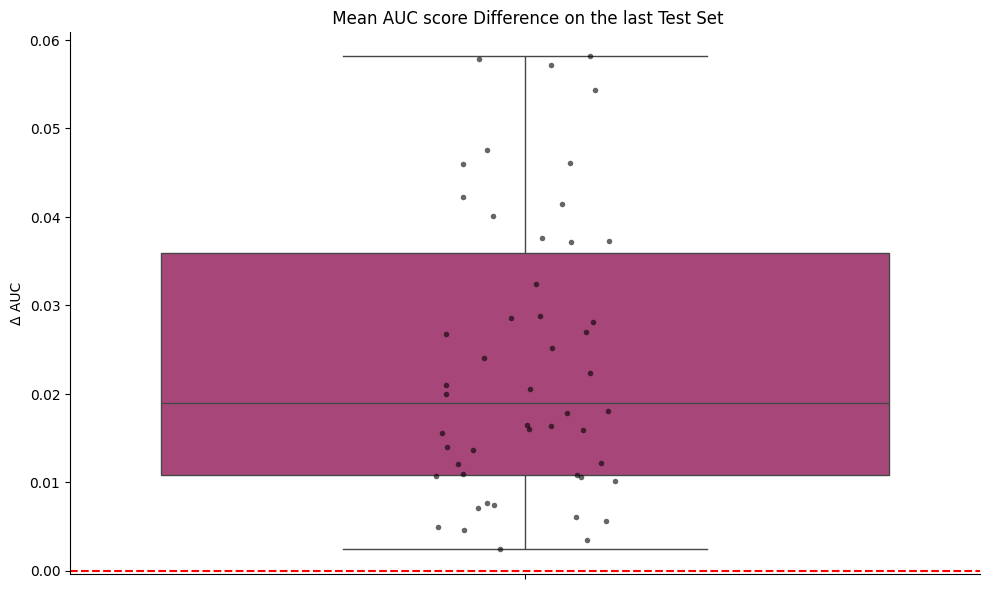
\includegraphics[width=\textwidth]{meandiffLAST.png}
            \end{figure}
        \end{column}
    \end{columns}

    \begin{table}
        \centering
        \small
        \begin{tabular}{lcccc}
            \toprule
            & $\Delta\bar{\mu}$ & t-stat & p-value & 95\% CI \\
            \midrule
            $\Delta\overline{\text{AUC}}$* & 0.0083 & 8.75  & $1.39 \times 10^{-11}$ & [0.006, 0.010] \\
            $\Delta\overline{\text{AUC}}_{\text{last}}$** & 0.0235 & 10.59 & $2.86 \times 10^{-14}$ & [0.019, 0.028] \\
            \bottomrule
        \end{tabular}
    \end{table}
    
    \begin{footnotesize}
        * Mean AUC score difference across all 10 shifted test sets. \\
        ** AUC score difference on the most shifted test set.
    \end{footnotesize}
\end{frame}


    
